\section{Projektmanagement}
Das PREN Modul ist ein Interdisziplinäres Modul. Von jeder der folgenden Fachrichtungen: Informatik, Elektrotechnik und Maschinenbau, ist mindestens eine Person pro Gruppe vertreten. Das Team 27 setzt sich wie folgt zusammen:
\begin{itemize}
	\item 3 Informatiker
	\item 3 Maschinenbauer
	\item 1 Elektrotechniker
\end{itemize}
Anfangs des Moduls wurden den Mitgliedern des Teams verschiedene Funktionen zugewiesen um eine Struktur und Ansprechpersonen innerhalb des Teams zu erhalten. Ersichtlich in folgendem Organigramm:
\begin{figure}[h!]
	\centering
	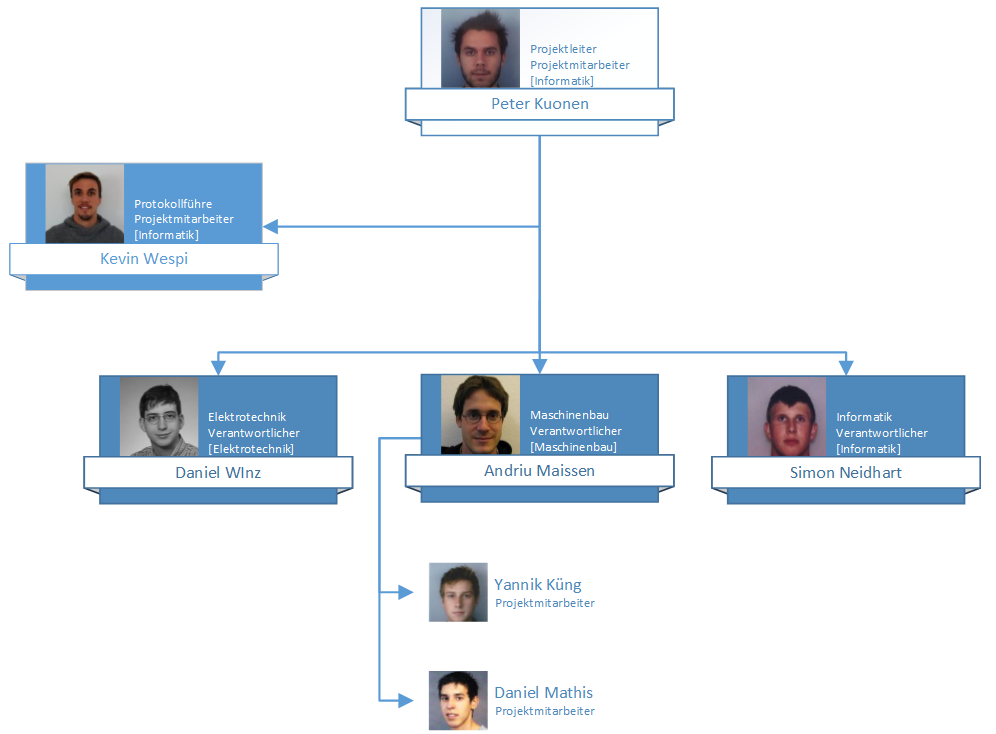
\includegraphics[width=0.7\textwidth]{fig/Organigramm.png}
	\caption{Organigramm}
	\label{fig:Organigramm}
\end{figure}

\subsection{Projektplanung}
Im folgenden wird die Planung mittels Zeitachsen für die jeweiligen Meilensteine dargestellt. In den folgenden Abbildungen sind diese dargestellt. Sie enthalten die Hauptaufgaben welche für die jeweiligen Meilensteine notwendig sind. Dies wurde angefertigt um die Übersicht über das Projekt zu haben und die verlangten Dokumente und Schritte zur Erfüllung der Meilensteine fristgerecht zu erledigen.



\begin{figure}[h!]
	\centering
	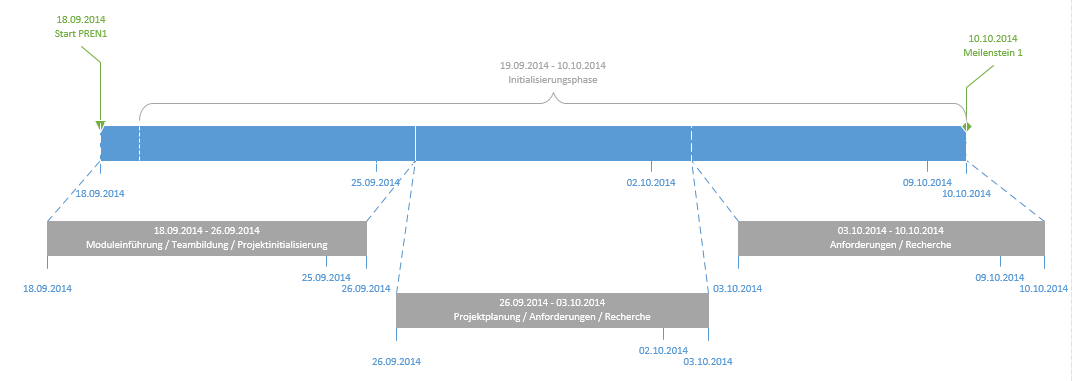
\includegraphics[width=1\textwidth]{fig/PlanungBisMS1.png}
	\caption{Planung Meilenstein 1}
	\label{fig:MS1}
\end{figure}
\begin{figure}[h!]
	\centering
	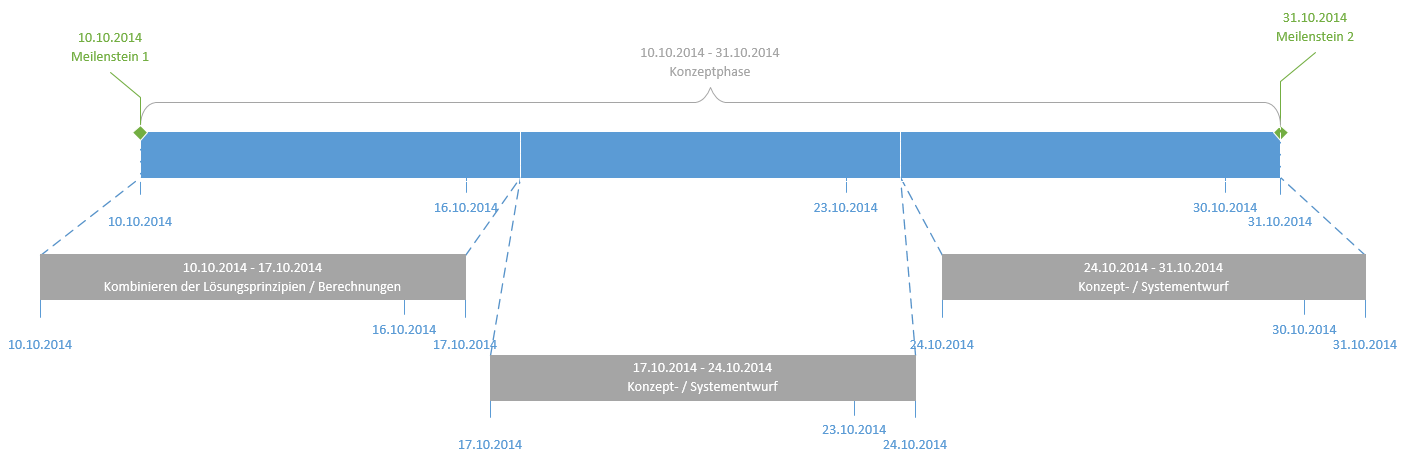
\includegraphics[width=1\textwidth]{fig/PlanungBisMS2.png}
	\caption{Planung Meilenstein 2}
	\label{fig:MS2}
\end{figure}
\begin{figure}[h!]
	\centering
	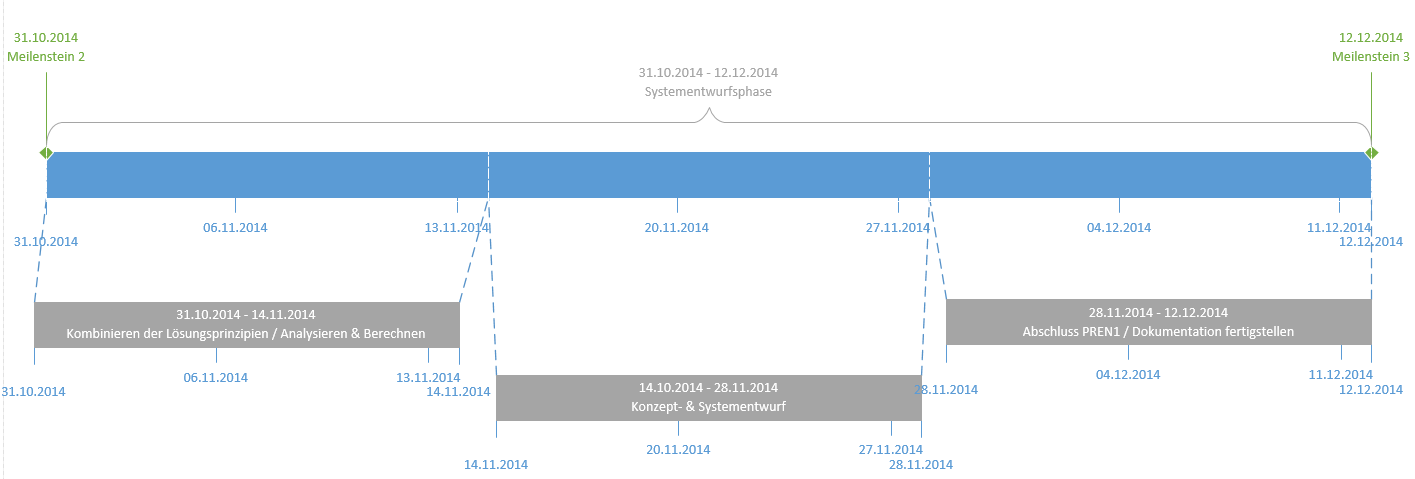
\includegraphics[width=1\textwidth]{fig/PlanungBisMS3.png}
	\caption{Planung Meilenstein 3}
	\label{fig:MS3}
\end{figure}